\documentclass[10pt,a4paper, margin=1in]{article}
\usepackage{fullpage}
\usepackage{amsfonts, amsmath, pifont}
\usepackage{amsthm}
\usepackage{graphicx}
\usepackage{pgfplots}

\usepackage{geometry}
 \geometry{
 a4paper,
 total={210mm,297mm},
 left=10mm,
 right=10mm,
 top=10mm,
 bottom=10mm,
 }
 % Write both of your names here. Fill exxxxxxx with your ceng mail address.
 \author{
  Özalp, Zeynep\\
  \texttt{e2237691@ceng.metu.edu.tr}
  \and
  Yıldırım, Hilmi Cihan\\
  \texttt{e2237949@ceng.metu.edu.tr}
}
\title{CENG 384 - Signals and Systems for Computer Engineers \\
Spring 2020 \\
Written Assignment 1}
\begin{document}
\maketitle



\noindent\rule{19cm}{1.2pt}

\begin{enumerate}

\item 
    \begin{enumerate}
    % Write your solutions in the following items.
    \item %write the solution of q1a
    \begin{enumerate}
    \item $\overline{z}=x-yj$ \\
    $z+1=j-3(x-yj) \Rightarrow z+1=j-3x+3yj \Rightarrow x+yj+1=j-3x+3yj$ \\
    $x+1=-3x \Rightarrow x=-1/4 \Rightarrow y=-1/2$ \\
    $z=-1/4-(1/2)j$\\
    $|z|^2=(-1/4-(1/2)j)*(-1/4+(1/2)j)=5/16$\\
    \item $z=-1/4-(1/2)j$\\
    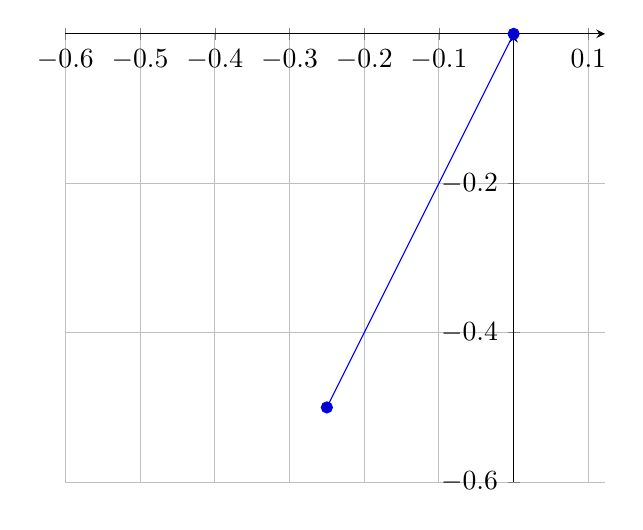
\begin{tikzpicture}{h}
\begin{axis}[axis lines=middle,axis equal, grid=both,xmin=-0.6, ymin=-0.6]
\addplot coordinates{(0,0) (-1/4,-1/2)};
\end{axis}
\end{tikzpicture}
    \end{enumerate}
    \item %write the solution of q1b
    z in polar form $z^2=r^2e^{2j\theta}=25j$ \\
    $r^2=cos2\theta+jsin2\theta=25j$ \\
    $cos2\theta=0$ and $sin2\theta=1\ then\ r=\pm5$, $\theta=\pi/4$\\
    $z=\pm5e^{j\pi/4}$
    \item %write the solution of q1c
   	z in polar form $\Rightarrow \dfrac{\sqrt{2}e^{j\pi/4}*2e^{-j\pi/3}}{\sqrt{2}e^{-j\pi/4}}=2e^{j\pi/6}$\\
   	magnitude is 2, angle is $\pi/6$.
    \item %write the solution of q1d
    $z=j(cos(-\pi/2)+jsin(-\pi/2))=-j^2=1 \Rightarrow z=e^{j2\pi k}$, $k=0,\pm1,\pm2...$
    \end{enumerate}


\item %write the solution of q2
.\\
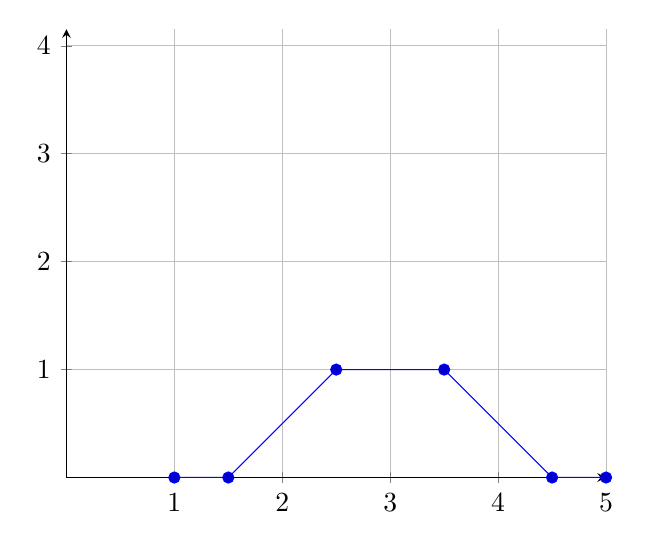
\begin{tikzpicture}{h}
\begin{axis}[axis lines=middle, axis equal, grid=both, xmin=0, ymin=0]
\addplot coordinates{(1,0) (3/2,0) (5/2,1) (7/2,1) (9/2, 0) (5,0)};
\end{axis}
\end{tikzpicture}

\item      
    \begin{enumerate}
    \item %write the solution of q3a
    
    \item %write the solution of q3b
    \end{enumerate}

\item 
    \begin{enumerate}
    \item %write the solution of q4a
    Yes. $N_0=48$.
    \item %write the solution of q4b
    \item %write the solution of q4c
    Yes. $T_0=3/5$
    \item %write the solution of q4d
    Yes. $T_0=\pi$
    \end{enumerate}

\item %write the solution of q5
Odd part of x(t): \\ 
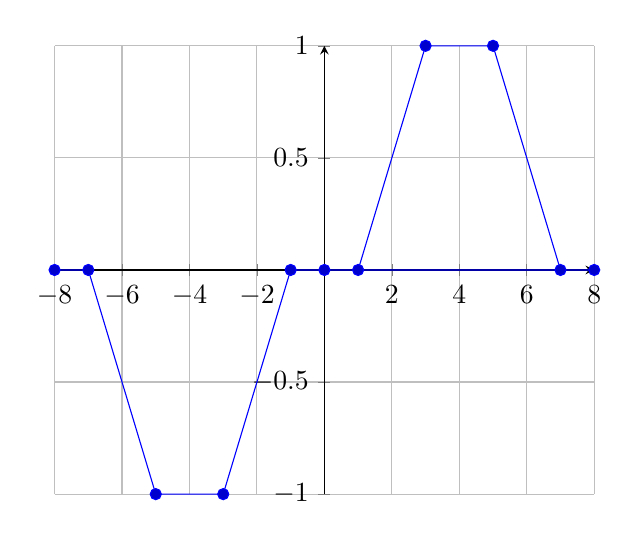
\begin{tikzpicture}{h}
\begin{axis}[axis lines=middle, grid=both, xmin=-8, ymin=-1]
\addplot coordinates{(-8,0) (-7,0) (-5,-1) (-3,-1) (-1,0) (0,0) (8,0) (7,0) (5,1) (3,1) (1,0)};
\end{axis}
\end{tikzpicture}

Even part of x(t): \\ 
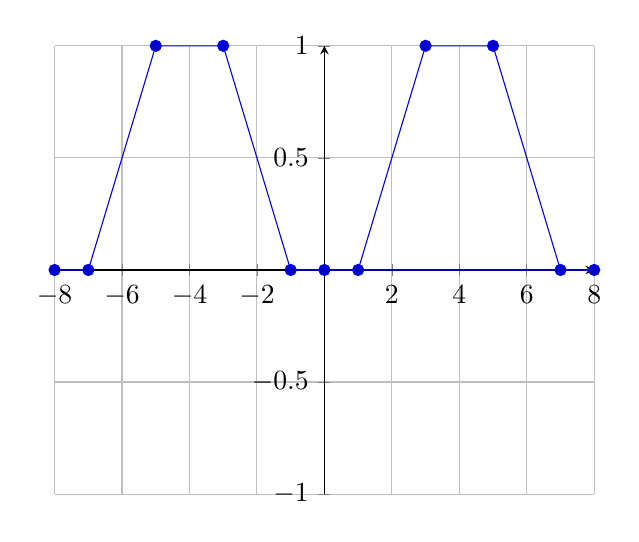
\begin{tikzpicture}{h}
\begin{axis}[axis lines=middle, grid=both, xmin=-8, ymin=-1]
\addplot coordinates{(-8,0) (-7,0) (-5,1) (-3,1) (-1,0) (0,0) (8,0) (7,0) (5,1) (3,1) (1,0)};
\end{axis}
\end{tikzpicture}

\item 
    \begin{enumerate}
    \item %write the solution of q6a
    $x(t)=\mu(t-1)-3\mu(t-3)+4\mu(t-4)$
    \item %write the solution of q6b
    $\dfrac{dx(t)}{dt}=\dfrac{d\mu(t-1)}{dt}-3\dfrac{d\mu(t-3)}{dt}+4\dfrac{d\mu(t-4)}{dt}=\delta(t-1)-3\delta(t-3)+4\delta(t-4)$
    \end{enumerate}
I could not draw arrows of unit impulse. So, I added triangles.\\
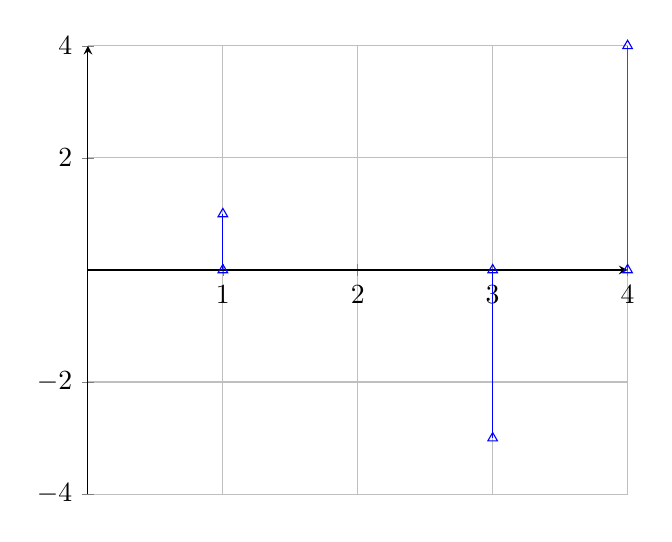
\begin{tikzpicture}{h}
\begin{axis}[axis lines=middle, grid=both, xmin=0, ymin=-4]
\addplot[mark=triangle, color=blue] coordinates{(1,0) (1,1)};
\addplot[mark=triangle, color=blue] coordinates{(3,0) (3,-3)};
\addplot[mark=triangle, color=blue] coordinates{(4,0) (4,4)};
\end{axis}
\end{tikzpicture}

\end{enumerate}
\end{document}

